\documentclass[../../main.tex]{subfiles}

\begin{document}

\section{Medición de capacitores}

\begin{figure}[H]	
	\centering
	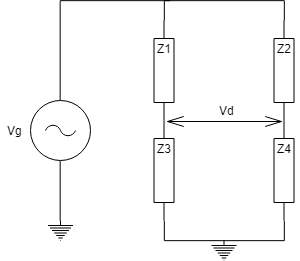
\includegraphics[width=0.35\textwidth]{fotos/PuenteGen.png}
	\caption{Puente con Impedancias ge\'nericas} \label{fig:pgc}
\end{figure}

Se diseñó un puente que permita medir capacitores en un rango de capacidad $C \in [10nF,100nF]$ y en un rango de factor de disipación $D \in[0.015 , 0.09 ] $, para una frecuencia de 10KHz. 
\par Partiendo del puente de la figura \ref{fig:pgc}, donde $V_d=\frac{Z_3}{Z_1+Z_3} -\frac{Z_4}{Z_4 + Z_2}$, en el equilibrio $Z_1 Z_4 = Z_2  Z_3$.  Reemplazando $Z_1= R_1 + \frac{1}{SC_1}$, $Z_2= R_x + \frac{1}{SC_x}$, $Z_3=R_3$ y $Z_4=R_4$. En el equilibrio se cumple que $C_x=\frac{C_1 R_3}{R_4}$, $R_x=\frac{R_1 R_4}{R_3}$ y $D_x=2 \pi f C_1 R_1$.

\subsection{Elección de componentes}
Fijando $C_1=3nF$ y $R_3=1K \Omega$, y a partir de las ecuaciones  $C_x=\frac{C_1 R_3}{R_4}$ y $D_x=2 \pi f C_1 R_1$, se obtuvieron los valores de las variables de ajuste, $R_1 \in \left[  \frac{D_{min}}{2 \pi f C_1 R_1} ,  \frac{D_{max}}{2 \pi f C_1 R_1}  \right] = \left[ 79.5\Omega , 477.46 \Omega   \right]$ y 
$R_4 \in \left[ \frac{C_1 R_3}{C_{Xmax}} , \frac{C_1 R_3}{C_{Xmin}} \right]=   \left[ 30\Omega , 300 \Omega   \right]$.
\par La resitencia $R_1$ se implementó con una resistencia de $68 \Omega$ en serie con dos presets de $200 \Omega$ y la resistencia $R_4$ se implementó con una resistencia de $20\Omega$ en serie con un preset de $200 \Omega$ y otro de $100 \Omega$.

\subsection{An\'alisis de sensibilidades}
Para analizar la sensibilidad del puente, se grafic\'o el cociente de la sensibilidad de $V_d$ respecto de $R_1$ y $R_2$.  El objetivo es que dicho cociente se encuentre lo mejor posible ditribuido entre 0 y 1.\par
Con los valores de los componentes indicados anterioremente se obtuvo el siguiente gr\'afico del cociente de las sensibilidades
\begin{figure}[H]	
	\centering
	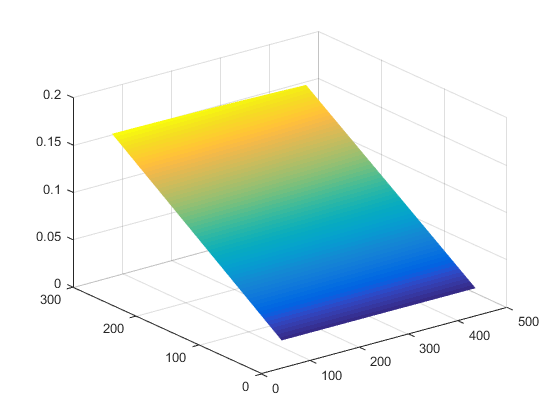
\includegraphics[width=0.7\textwidth]{fotos/sen.png}
	\caption{Cociente de sensibilidades} 
\end{figure}
Como se observa en el gr\'afico, al variar $R_1$ y $R_4$ se obtuvo una superficie acotada entre 0 y 1.

\subsection{Calculo del error}
Para calcular el error en la medici\'on se tuvo que distinguir cu\'ales fueron las fuentes de error en la medici\'on. Supusimos que el error en analizador de impedancias es despreciable.\par
Las fuentes de error que supusimos fueron las siguientes:
\begin{itemize}  
\item El error en la medición de las resistencias por parte del \'ohmetro lo consideramos de $1\Omega$
\item Como $V_d$ nunca llega a cero, y como la medici\'on se realiz\'o con el volt\'imetro de banco consideramos que el error en la medici\'on de $V_d$ es de 1mV 
\end{itemize}

Conociendo que constructivamente $R_1$ y $R_4$ se realizaron con presets de $200\Omega$, estimamos el $\Delta R_1=\Delta R_2=2\Omega$ (un cuarto de vuelta del preset).

$$S_{R_1}^{V_d} \Delta R_1=\Delta V_d$$
$$\Delta R_1 = 8\Omega$$

Considerando el peor caso cuando se suman los errores, para $\Delta R_1 = 8\Omega$, ahora calculamos para $C_x$.
$$\Delta C_x = C_1 R_3 \frac{\Delta R_4}{R_4^2} $$
Como en el peor caso $R_4=30\Omega$
$$\Delta C_x=3nF $$
Y por \'ultimo, hay que hallar el error en $D_x$. Como $D_x=2\pi f  C_1 R_1$, entonces:
$$ \Delta D_x= 2 \pi  f  C_1 \cdot \Delta R_1 $$
$$ \Delta D_x=0.0009$$

\subsection{Convergencia}
Se analiz\'o si el puente converg\'ia para un \'unico valor de $R_1$ a un \'unico $D_x$ y $R_4$ a un \'unico $C_x$. Para ello se grafic\'o Vd en funcion de $C_x$ y $R_4$ en un caso y $R_1$ , $D_x$ para el otro.

\begin{figure}[H]	
	\centering
	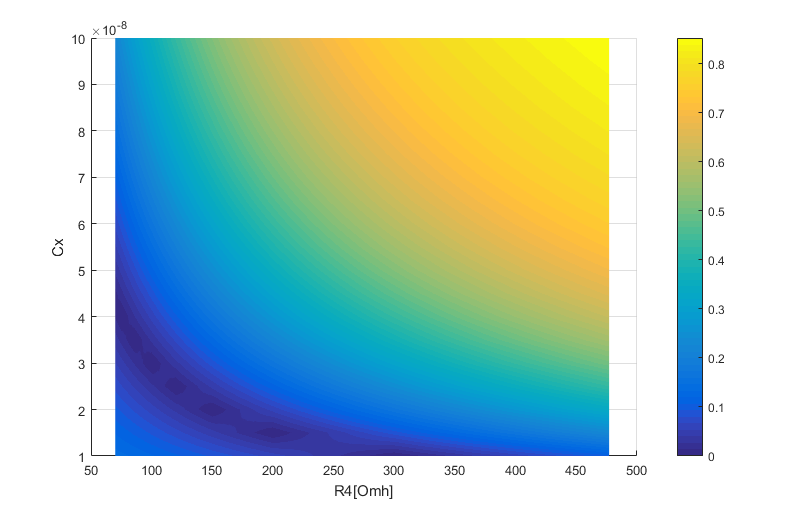
\includegraphics[width=0.7\textwidth]{fotos/conv_cx.png}
	\caption{Convergencia de $V_d$ respecto de $R_4$ y $C_x$ } 
\end{figure}

\begin{figure}[H]	
	\centering
	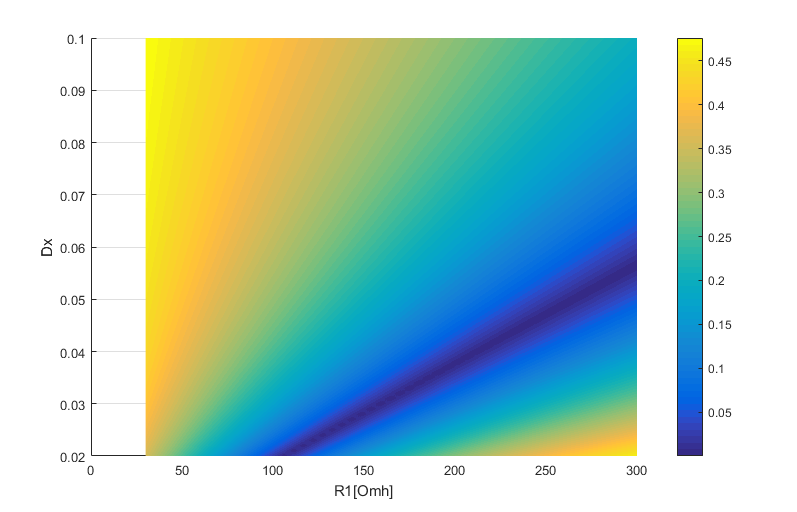
\includegraphics[width=0.7\textwidth]{fotos/conv_dx.png}
	\caption{Convergencia de $V_d$ respecto de $R_1$ y $D_x$ } 
\end{figure}

Como se observa en ambas figuras hay una unica franja violeta (m\'inimo) de $V_d$, por ende la convergancia del puente es unica para cada $C_x$ y $D_x$.

\subsection{Manual de uso}
Para poder medir en el puente, se recomienda primero ajustar el preset correspoendiente a $R_4$, debido a que la sensibilidad del puente es mayor respecto a dicha reisitencia, encontrando el m\'inimo de $V_d$. Despu\'es variar $R_1$ para minimizar a\'un mas $V_d$. Posteriormente desconectar todos los elementos del puente y medir las resistencias $R_4$ y $R_1$. Finalmente con las ecuaciones anteriormente mencionadas se obtiene el valor del capacitor medido, donde $C_x=\frac{C_1 R_3}{R_4}$, $R_x=\frac{R_1 R_4}{R_3}$ y $D_x=2 \pi f C_1 R_1$.

\subsection{Mediciones}
Se midieron los capacitores con el analizador de impedancias y con el puente.

\subsubsection{Analizador de impedancia}

\begin{table}[H]
\begin{center}
\begin{tabular}{|c|c|c|}
\hline
 Frecuencia&C&D\\
\hline \hline

$ 1KHz$ &9.8nF&0.015  \\ \hline
$ 10KHz$  & 9.6nF&0.023  \\ \hline
$ 100KHz$  &9.3nF &0.085  \\ \hline

\end{tabular}
\caption{Capacitor m\'inimo } 
\end{center}
\end{table}
\begin{table}[H]
\begin{center}
\begin{tabular}{|c|c|c|}
\hline
 Frecuencia&C&D\\
\hline \hline

$ 1KHz$ &47.24nF&0.019  \\ \hline
$ 10KHz$  & 26nF&0.003 \\ \hline
$ 100KHz$  &43.56nF &0.08  \\ \hline

\end{tabular}
\caption{Capacitor medio} 
\end{center}
\end{table}

\begin{table}[H]
\begin{center}
\begin{tabular}{|c|c|c|}
\hline
 Frecuencia&C&D\\
\hline \hline

$ 1KHz$ &108nF&0.018  \\ \hline
$ 10KHz$  & 108nF&0.024  \\ \hline
$ 100KHz$  &102nF &0.083  \\ \hline

\end{tabular}
\caption{Capacitor m\'aximo } 
\end{center}
\end{table}

\begin{table}[H]
\begin{center}
\begin{tabular}{|c|c|c|}
\hline
 Frecuencia&C&D\\
\hline \hline

$ 1KHz$ &186nF&0.01  \\ \hline
$ 10KHz$  & 181nF&0.016  \\ \hline
$ 100KHz$  &171nF &0.08  \\ \hline

\end{tabular}
\caption{Capacitor doble del m\'aximo } 
\end{center}
\end{table}



\subsubsection{Puente}
Se midió $V_d$ con el volt\'imetro de banco

\begin{table}[H]
\begin{center}
\begin{tabular}{|c|c|c|}
\hline
 Frecuencia&C&D\\
\hline \hline

$ 1KHz$ &9.87nF&0.005  \\ \hline
$ 10KHz$  & 9.9nF&0.013  \\ \hline
$ 100KHz$  &9.58nF &0.1  \\ \hline

\end{tabular}
\caption{Capacitor m\'inimo } 
\end{center}
\end{table}
\begin{table}[H]
\begin{center}
\begin{tabular}{|c|c|c|}
\hline
 Frecuencia&C&D\\
\hline \hline

$ 1KHz$ &44.8nF&0.0013  \\ \hline
$ 10KHz$  & 45.5nF&0.012 \\ \hline
$ 100KHz$  &42.4nF &0.13  \\ \hline

\end{tabular}
\caption{Capacitor medio } 
\end{center}
\end{table}

\begin{table}[H]
\begin{center}
\begin{tabular}{|c|c|c|}
\hline
 Frecuencia&C&D\\
\hline \hline

$ 1KHz$ &108nF&0.0013  \\ \hline
$ 10KHz$  & 108nF&0.013  \\ \hline
$ 100KHz$  &89.6nF & 0.14 \\ \hline

\end{tabular}
\caption{Capacitor m\'aximo } 
\end{center}
\end{table}

\begin{table}[H]
\begin{center}
\begin{tabular}{|c|c|c|}
\hline
 Frecuencia&C&D\\
\hline \hline

$ 1KHz$ &115nF&0.003  \\ \hline
$ 10KHz$  & 115nF&0.037  \\ \hline
$ 100KHz$  &115nF &0.3  \\ \hline

\end{tabular}
\caption{Capacitor doble del m\'aximo } 
\end{center}
\end{table}



\subsection{Conclusión}
Como era de esperarse la medicion del capacitor al doble del maximo, no se puedo medir debido que el preset lleg\'o a su maximo. En cuanto a la medicion del $D$ del capacitor en todos los casos nos dio mal, esto atribuimos a un errado analisis de sensibilidades, y esto implic\'o que al variar el preset correspondiente al $D$ no se pudiese apreciar una variacion en el $V_d$. Adem\'as para mejorar la medición se tendria que haber medido con un amplificador de instrumentación.



\end{document}

